%\documentclass[a4paper,12pt]{report}
\documentclass[a4paper,12pt]{article}
%\documentclass[a4paper,12pt]{book}
\usepackage{polski}
\usepackage[polish]{babel}
\usepackage[utf8]{inputenc}
\usepackage[top=2.5cm, bottom=2.5cm, left=3cm, right=2.5cm]{geometry}
\usepackage{graphicx}
\usepackage{setspace}
\usepackage{ifthen}
%\usepackage[utf8]{inputenc}
\usepackage{a4wide}
\usepackage{fullpage}
\usepackage{verbatim}
\usepackage[usenames,dvipsnames]{color}
\usepackage{hyperref}
\usepackage{subfig}
\usepackage{listings}
\usepackage{mdwlist}
\usepackage{titlesec}
\usepackage{lipsum}

\hypersetup{
	bookmarks=true,
%	pdftitle={INŻ; Projekt – Sprawozdanie},
	pdftitle={EtherCAT},
	pdfauthor={Damian Karbowiak},
	pdfsubject={EtherCAT},
	pdfkeywords={INŻ sprawozdanie Politechnika Śląska EtherCAT raport końcowy projekt magisterski},
	colorlinks=true,
	linkcolor=Black,
	citecolor=Black,
	urlcolor=Black
	}

\let\subsubsubsection\paragraph
%\setcounter{secnumdepth}{6} % subsubparagraph ???
% that is, subsubsubsubsubsection :-)
\setcounter{secnumdepth}{4}

\newcommand{\tytul}{System sterowania i wizualizacji pracy robota 3D}
\newcommand{\data}{czerwiec 2013}
\newcommand{\promotor}{dr~inż. Jacek Stój}
\newcommand{\autor}{Damian Karbowiak}
%\newcommand{\konsultant}{mgr inż. Wojciech Domagała }
\newcommand{\konsultant}{}

\titlespacing{\section}{1cm}{*4}{*1.5}
\titlespacing{\subsection}{1cm}{*4}{*1.5}
\titlespacing{\subsubsection}{1cm}{*4}{*1.5}

\begin{document}
\lstset{backgroundcolor=\color{white}, boxpos=c, captionpos=b}
\lstset{numbers=left, stepnumber=1, numbersep=10pt, frame=single}
\lstset{frameround=tttt}
\renewcommand{\lstlistlistingname}{\vspace*{-13mm}}
\renewcommand{\listfigurename}{\vspace*{-13mm}}
%\renewcommand*\l@figure[2]{\indent}
\renewcommand{\listtablename}{\vspace*{-13mm}}
\renewcommand*{\refname}{\vspace*{-13mm}}
\renewcommand{\lstlistingname}{Kod źródłowy} 

\begin{titlepage}
  \begin{center}
    \vspace*{5.1mm}
    
\includegraphics[width=3.41cm]{logo}
    \vskip 1.58cm
    \scalebox{0.93}{\textbf{\uppercase{\textsf{\Large P{\large olitechnika} Ś{\large lĄska}}}}}
    \vskip 6.1mm
    \scalebox{0.93}{\textbf{\uppercase{\textsf{\Large W{\large ydziaŁ} A{\large utomatyki}, E{\large lektroniki} {\large i} I{\large nformatyki}}}}}
    \vskip 4.6mm
    %\scalebox{0.93}{\textbf{\uppercase{\textsf{\Large K{\large ierunek} I{\large nformatyka}}}}}
    {\textbf{\uppercase{\textsf{\large K{\normalsize ierunek} I{\normalsize nformatyka}}}}}
    \vskip 2.3cm
    \textsf{\LARGE Praca dyplomowa magisterska}
    \vskip 1.8cm
    \begin{onehalfspace}
      \textsf{\large \tytul}
    \end{onehalfspace}
  \end{center}
  \vfill

  \noindent\textsf{\large Autor: \autor}
  \vskip 3mm
  \noindent\textsf{\large Kierujący pracą: \promotor}
  \ifthenelse{\equal{\konsultant}{}}{
    \vskip 36mm
  }{
    \vskip 3mm
    \noindent\textsf{\large Konsultant: \konsultant}
    \vskip 27.7mm
  }
  \noindent\textsf{Gliwice, \data}
  \vspace*{2mm}
\end{titlepage}
 %

\tableofcontents
\addtocontents{toc}{\protect\vspace*{.05\baselineskip}}
\clearpage

\section{Wstęp}
Tematem, którego dotyczy ta praca jest: „Projekt i~realizacja stanowiska laboratoryjnego do badania zależności czasowych w~sieci EtherCAT". Zagadnienia związane z~tworzeniem oprogramowania dla sterowników przemysłowych są dla autora niezwykle interesujące, a zrealizowany projekt miał na~celu dalsze pogłębienie jego wiedzy z~tego zakresu. Wyboru tego konkretnego tematu autor dokonał, ponieważ protokół EtherCAT jest jeszcze nowością i~według wielu źródeł stanowi przyszłość branży informatyki przemysłowej \cite{art1_etherCAT, art2_etherCAT}, a~praca nad tym tematem wydaje się być pomocna i~wartościowa w~przyszłej pracy zawodowej lub na~ewentualnym dalszym etapie kształcenia.

\subsection{Geneza}
Informatyka przemysłowa to dziedzina wiedzy z~pogranicza nauk informatycznych oraz szeroko pojętych nauk o~technologiach przemysłowych łącząca te~dwa zakresy wiedzy. Informatyka przemysłowa to~dział, który jest niezwykle pomocny, zwłaszcza przy analizach danych, ale~również podczas tworzenia funkcjonalnych i~wydajnych maszyn dla nowoczesnych gałęzi gospodarki. Specjaliści z~zakresu informatyki przemysłowej zajmują się takimi zagadnieniami jak monitorowanie produkcji przemysłowej czy też analizowaniem wybranych danych, które później służą do~porównań. Niezwykle ważne jest wykorzystanie tych danych, które dostarczą istotnych informacji dla każdego przemysłu, a~także sterowanie produkcji przemysłowej, która pomaga w~dynamicznym rozwoju każdej gałęzi w~gospodarce. 
Przemysł to~szczególna gałąź gospodarki, która aby się rozwijać potrzebuje nowoczesnych rozwiązań. Jedną z~nich jest informatyka, która pozwala na~udoskonalanie wyprodukowanych już maszyn przemysłowych, a~także tych, które dopiero są w~trakcie rozwoju technologicznego. Informatyka to aspekt, który zwraca uwagę na~nowoczesne zastosowanie komputerów w~celach przemysłowych. Wielu informatyków współpracuje z~firmami działającymi w~przemyśle, gdyż współpraca opłaca się obydwu stronom.

Systemy komputerowe realizują bardzo odpowiedzialne zadania, a~współczesna technologia stawia coraz poważniejsze wymagania związane przede wszystkim z~gwarantowanym i~nieprzekraczalnym czasem realizacji pojedynczego cyklu sterowania bądź regulacji, co wymaga wprowadzenia rozwiązań gwarantujących determinizm czasowy. Determinizm czasowy oznacza, że wyniki działania systemu komputerowego pojawiają się w~określonym i~skończonym czasie.

\subsection{Przemysłowe systemy czasu rzeczywitego}
System czasu rzeczywistego (ang. \textit{Real-Time System}, w~skrócie \textit{RTS}) według jednej z~definicji jest to~system komputerowy, w~którym obliczenia są prowadzone równolegle z~przebiegiem zewnętrznego procesu w~otoczeniu systemu (w~sterowanym obiekcie). Mają one na celu nadzorowanie, sterowanie oraz terminowe reagowanie na~zdarzenia zachodzące w~tym procesie. Uproszczony schemat działania przedstawiono na~Rysunku~\ref{wstep:rts}.
\begin{figure}[htbp]
 \centering
        \tikzstyle{background grid}=[draw, black!50,step=.25cm]
	\begin{tikzpicture}[node distance=1cm, auto]%, show background grid]
	\tikzset{
    	mynode/.style={rectangle,rounded corners,draw=black, fill=white!15,very thick, inner sep=0.9em, minimum size=2.5em, 		text centered, text width=2.5cm},
	    myarrow/.style={->, >=latex', shorten >=1pt, ultra thick},
	    myline/.style={-, =latex', shorten >=1pt, rounded corners, ultra thick},
	    mylabel/.style={text width=7em, text centered} 
	} 
	\node[mynode] (device2) {Obiekt (otoczenie)};  
	\node[mynode, fill=white!15, left=5cm of device2] (device1) {System \\ czasu \\ rzeczywistego};
	\node[right=0.1cm of device2] (loop) {};
	
	\draw[myarrow] ([yshift=6mm]device2.west) -- ([yshift=6mm]device1.east) node [midway,yshift=3.5mm,fill=white] {Zdarzenia};		
		\draw[myarrow] ([yshift=0mm]device2.west) -- ([yshift=0mm]device1.east) node [midway,yshift=3.5mm,fill=white] {Stan systemu};
	\draw[myarrow] ([yshift=-6mm]device1.east) -- ([yshift=-6mm]device2.west) node [midway,yshift=-3.5mm,fill=white] {Odpowiedzi};		
 
\end{tikzpicture} 
\caption{Schemat działania systemu czasu rzeczywistego.}
\label{wstep:rts}
\end{figure} %
\vspace{-3mm}

System czasu rzeczywistego jest takim systemem, który do poprawnego działania musi spełniać następujące warunki:
\begin{enumerate}
\item Warunki logiczne -- odpowiedź systemu musi być zawsze prawidłowa przy uwzględnieniu stanu systemu, tzn. odpowiedź zależy od stanu otoczenia i~występujących zdarzeń oraz jest zgodna z~założeniami technologicznymi,
\item Warunki czasowe -- odpowiedź systemu musi nadejść we właściwym czasie (przed przekroczeniem czasu granicznego dla danego systemu).
\end{enumerate}

\tikzset{
%Define standard arrow tip
>=stealth',
%Define style for different line styles
help lines/.style={dashed, thick},
axis/.style={<->},
important line/.style={thick},
connection/.style={thick, dotted},
}
\newcommand\A{\ensuremath{\mathcal{A}}}
\newcommand\B{\ensuremath{\mathcal{B}}}

\begin{figure}[htbp]
 \centering
	\subfloat[System typu ,,hard'']{
		\label{wstęp:funkcja_zysku:1}	
		\begin{tikzpicture}

		% horizontal axis
		\draw[->] (0,0) -- (5,0) node[anchor=north] {$t$};
		% labels
		\draw	(1.1,0) node[anchor=north east] {$t_0$}
				(3,0) node[anchor=north east] {$t_T$};
		
		% vertical axis
		\draw[->] (0,-1) -- (0,3) node[anchor=east] {$z(t)$};
		% labels
		\draw	(0.1,1.9) node[anchor=south east] {$u$}
				(0,-1.2) node[anchor=south east] {$-\infty$};
						
		% ciągłe
		\draw[ultra thick] (1,2) -- (3,2);
		
		% Przerywane
		\draw[thick,dashed] (-0.2,2) -- (1,2);
		\draw[thick,dashed] (1,-0.2) -- (1,2);
		\draw[ultra thick,dashed, <-] (3,-0.9) -- (3,2);		
		
		\draw (8,1.5) node {
		$z(t)=\left\{
			\begin{array}{c l}     
			    u & t_0<t<t_T\\
		       -\infty & t \geq t_T
			\end{array}\right.$ };
					
		\end{tikzpicture}	
	}                
	
	\subfloat[System typu ,,firm'']{ 
		\label{wstęp:funkcja_zysku:2}
		\begin{tikzpicture}

		% horizontal axis
		\draw[->] (-0.2,0) -- (5,0) node[anchor=north] {$t$};
		% labels
		\draw	(1.1,0) node[anchor=north east] {$t_0$}
				(3,0) node[anchor=north east] {$t_T$};
		
		% vertical axis
		\draw[->] (0,-0.5) -- (0,3) node[anchor=east] {$z(t)$};
		% labels
		\draw	(0.1,1.9) node[anchor=south east] {$u$}
				(0,-0.1) node[anchor=south east] {$0$};
						
		% ciągłe
		\draw[ultra thick] (1,2) -- (3,2);
		\draw[ultra thick, ->] (3,0) -- (5,0);		
		
		% Przerywane
		\draw[thick,dashed] (-0.2,2) -- (1,2);
		\draw[thick,dashed] (1,-0.2) -- (1,2);
		\draw[ultra thick,dashed] (3,0) -- (3,2);		
		
		\draw (8,1.5) node {
		$z(t)=\left\{
			\begin{array}{c l}     
			    u & t_0<t<t_T\\
		        0 & t \geq t_T
			\end{array}\right.$ };
			
		\end{tikzpicture}		
	}
	
	\subfloat[System typu ,,soft'']{
		\label{wstęp:funkcja_zysku:3}	
		\begin{tikzpicture}

		% horizontal axis
		\draw[->] (-0.2,0) -- (5,0) node[anchor=north] {$t$};
		% labels
		\draw	(1.1,0) node[anchor=north east] {$t_0$}
				(2.1,0) node[anchor=north east] {$t_1$}
				(3,0) node[anchor=north] {$t_T$};
		
		% vertical axis
		\draw[->] (0,-0.5) -- (0,3) node[anchor=east] {$z(t)$};
		% labels
		\draw	(0.1,1.9) node[anchor=south east] {$u$}
				(0,-0.1) node[anchor=south east] {$0$};
						
		% ciągłe
		\draw[ultra thick] (1,2) -- (2,2);
		\draw[ultra thick] (2,2) -- (3,0);		
		\draw[ultra thick, ->] (3,0) -- (5,0);		
		
		% Przerywane
		\draw[thick,dashed] (-0.2,2) -- (1,2);
		\draw[thick,dashed] (1,-0.2) -- (1,2);
		\draw[thick,dashed] (2,-0.2) -- (2,2);		

		\draw (8,1.5) node {
		$z(t)=\left\{
			\begin{array}{c l}     
			    u & t_0<t<t_1\\
			    u \frac{t_T-t}{t_T-t_1} & t_1<t<t_T\\
		        0 & t \geq t_T
			\end{array}\right.$ };
			
		\end{tikzpicture}
	}
\caption{Funkcja zysku dla systemów czasu rzeczywistego}
\label{wstep:funkcja_zysku}
\end{figure} %

Jak wynika z~przedstawionych na Rysunku~\ref{wstep:funkcja_zysku} teoretycznych funkcji zysku, rozróżniamy trzy typy systemów czasu rzeczywistego:
\begin{itemize}
\item systemy o~ostrych ograniczeniach czasowych (ang. \textit{hard real-time}) -- gdy przekroczenie terminu powoduje poważne, a~nawet katastrofalne skutki, jak np.~zagrożenie życia lub~zdrowia ludzi, uszkodzenie lub~zniszczenie urządzeń, przy czym nie~jest istotna wielkość przekroczenia terminu a~jedynie sam fakt jego przekroczenia. Wynika z~tego, ze informacja wygenerowana przez system po~przekroczeniu czasu granicznego $t_T$ oznacza poważny błąd systemu,

\item systemy o~mocnych ograniczeniach czasowych (ang. \textit{firm real-time}) -- gdy fakt przekroczenia terminu powoduje całkowitą nieprzydatność wypracowanego przez system wyniku, jednakże nie oznacza to zagrożenia dla ludzi lub sprzętu; pojęcie to stosowane jest głównie w~opisie teoretycznym baz danych czasu rzeczywistego,

\item systemy o~miękkich lub~łagodnych ograniczeniach czasowych (ang. \textit{soft real-time}) -- gdy przekroczenie pewnego czasu powoduje negatywne skutki tym poważniejsze, im~bardziej ten czas został przekroczony; w~tym przypadku przez ,,negatywne skutki'' rozumie się spadek funkcji zysku aż~do~osiągnięcia wartości zero.
\end{itemize}

Dla określenia podziału systemów czasu rzeczywistego przydatne jest pojęcie funkcji zysku \cite{rts}. Jest to funkcja zależna głównie od czasu i~dokonuje odwzorowania czasu wykonania zadania na korzyść wynikającą z~jego wykonania. Wartość korzyści niekoniecznie jest wielkością wymiarowaną. Źródłem występujących ograniczeń czasowych są~zazwyczaj zjawiska fizyczne zachodzące w~świecie rzeczywistym kontrolowanym przez system. Zadanie jest uznawane za~zrealizowane jako poprawne, jeśli w~chwili jego zakończenia wartość funkcji zysku jest większa od zera.
\clearpage
Założenia dla wykresów funkcji zysku \cite{rts}:
\begin{itemize}
\item $t_0$ -- jest to moment w~którym zadanie zostało zlecone oraz rozpoczęło się jego wykonywanie,
\item $t_T$ -- jest to graniczny moment w~którym przetwarzanie może zostać zakończone,
\item w~przypadku jak na Rysunku~\ref{wstęp:funkcja_zysku:3} funkcja z(t) jest funkcją ciągłą w~punktach $t_1$ i~$t_T$,
\item dla wartości $t \leq t_0$ funkcji zysku nie wyznacza się, gdyż jest to~sytuacja niemożliwa, tzn. obliczany byłby zysk z~zakończenia zadania przed jego rozpoczęciem, co~nie~może się zdarzyć i~nie ma sensu logicznego.
\end{itemize}

W tego typu systemach przekształcanie danych wymienianych między nim, a środowiskiem zewnętrznym zachodzi w~deterministycznie określonym czasie. W~opisach stosuje się pojęcie terminu (ang. \textit{deadline}), oznaczające najdłuższy dopuszczalny czas reakcji systemu na~wystąpienie zdarzenia \cite{rts}. Szybkość działania systemu czasu rzeczywistego nie~jest tak naprawdę ważna, istotne jest, aby spełnione były bezwarunkowo przyjęte ograniczenia czasowe.

Idealnymi przykładami praktycznymi z~życia codziennego wyjaśniającymi wprowadzony podział oraz funkcję zysku~są:
\begin{itemize}
\item W~przypadku systemów typu  ,,hard real-time'' jest to reaktor jądrowy. Zakładając, że system nadzorujący pracę takiego urządzenia nie~zdążyłby wystarczająco szybko zareagować na~podnoszenie się temperatury rdzenia i~doszłoby do~jego przegrzania lub nawet do~ częściowego stopienia. Jak pokazał przykład awarii reaktora jądrowego w~Czarnobylu tego typu zjawiska mają tragiczne i~wieloletnie skutki. Jest to~idealny przykład, że~nie pojawienie się odpowiedzi systemu na~czas może przynieść poważne konsekwencje i~nie~ma znaczenia o ile czas graniczny został przekroczony,
\item W~przypadku systemów typu  ,,soft real-time'' jest to bankomat. Jak wiadomo bankomat musi zareagować na~żądania zgłaszane przez klienta w~skończonym czasie. Jeżeli czas ten będzie zbyt długi, tzn. będzie przekraczał czas graniczny to~negatywnym skutkiem będzie spadające zadowolenie klienta wynikające z~jakości świadczonej usługi. Wiadomo, że~nie~wolno ignorować tego faktu, bo~niezadowolenie klienta może spowodować, że~nie~skorzysta on~więcej z~danej sieci bankomatów. Na~tym przykładzie dobrze widać, że przekroczenie czasu granicznego nie~jest poważne w~skutkach, ale powoduje spadek wartości funkcji zysku, którą jest w~tym przypadku zadowolenie klienta.
\end{itemize}
\clearpage
Systemy czasu rzeczywistego najczęściej pracują pod kontrolą specjalnych systemów operacyjnych spełniających reżimy czasu rzeczywistego. System operacyjny czasu rzeczywistego (ang. \textit{Real-Time Operating System}, w~skrócie \textit{RTOS}) jest to system operacyjny, który został opracowany tak, aby~spełniać wymagania narzucone na~czas wykonania zadanych operacji. Podstawowym wymaganiem dla systemu typu RTOS jest określenie najdłuższego możliwego czasu, po którym urządzenie wypracuje odpowiedź na wystąpienie zdarzenia (określenie przypadku pesymistycznego). 
%Ze względu na~kryterium ograniczeń czasowych systemy te~dzielimy na:
%\begin{itemize}
%\item Twarde (ang. \textit{Hard RTOS}) -- są to systemy, dla których znany jest najdłuższy i~nie przekraczalny gwarantowany czas odpowiedzi,
%\item Miękkie (ang. \textit{Soft RTOS}) -- są to systemy, które starają się odpowiedzieć w~możliwie najkrótszym czasie, ale niestety nie jest znany najdłuższy możliwy czas odpowiedzi.
%\end{itemize}

Zaawansowanym problemem występującym w~systemach operacyjnych tego typu jest dobór algorytmu szeregowania oraz przydziału czasu. W~systemie czasu rzeczywistego ze względu na ograniczone zasoby trzeba wybrać, który z~procesów będzie miał w~danym momencie przydzielony procesor oraz jak~długo przydział taki powinien trwać, aby wszystkie wykonywane procesy spełniły określone dla nich ograniczenia czasowe.

%Na rynku dostępnych jest aktualnie wiele systemów operacyjnych czasu rzeczywistego od różnych producentów lub otwartych, których przykłady przedstawia Tabela~\ref{rtos}.
%\begin{table}[!htb]
%\begin{center}
%\begin{tabular}{| p{0.03\textwidth} | p{0.17\textwidth} | p{0.3\textwidth} | p{0.4\textwidth} |}\hline
%\textbf{Nr} & \textbf{Nazwa} & \textbf{Producent} & \textbf{Platformy} \\\hline\hline
%1 & Solaris & Sun Microsystems & Sparc \\\hline
%2 & Windows CE & Microsoft & ARM, MIPS, PowerPC, SH, x86, Strong ARM, NEC, VR4111 \\\hline
%3 & QNX Neutrino & QNX Software Systems & MIPS, MPC8xx, PowerPC, SH, ARM, Strong~RM \\\hline
%4 & RT Linux & Open Source & ARM, PowerPC, x86, SH3, MIPS \\\hline
%5 & LynxOS & LynuxWorks & 68K, MIPS, MPC8xx, PowerPC, x86, Sparc \\\hline
%6 & VxWorks & Wind River Systems & 68K, i869, ARM, MIPS, PowerPC, x86, SH, SPARC \\\hline
%7 & eCOS & Open Source & ARM, MIPS, MPC8xx, PowerPC, Sparc \\\hline
%\end{tabular}
%\end{center}
%\vspace*{-6mm}
%  \caption{Systemy czasu rzeczywistego}
%	\label{rtos}
%\end{table}

Kolejnym niezbędnym elementem, oprócz układów wejściowych i~wyjściowych oraz kontrolowanych urządzeń (np. robotów) są deterministyczne sieci transmisyjne.
W~sieciach przemysłowych dane są~często przesyłane, ale~są~one krótkie (mają niewielki rozmiar), w~przeciwieństwie do~sieci ogólnego przeznaczenia, gdzie przesyła się dane rzadko~i~w~dużej ilości. Dane mają charakter np. wartości
pomiaru, rozkazów start/stop, alarmu, przekazania wartości zadanej do~zrealizowania przez regulator itd. Bardzo często informacja przesyłana w~tych sieciach ma rozmiar pojedynczego bitu lub słowa.

W~sieciach, w~których zagwarantowany jest determinizm czasowy transmisji, okres od wysłania pakietu danych od~nadawcy do~jego odbioru po~stronie odbiorcy jest z~góry znany i~pozostaje niezmienny. Wówczas komunikacja między węzłami sieci może być realizowana w~czasie rzeczywistym, łatwiejsza jest też ich synchronizacja. Obie te kwestie są kluczowe dla sprawnego działania systemów sterowania. Dodatkowo sieci takie muszą zapewniać wszelkiego rodzaju mechanizmy kontroli poprawności przesyłu danych oraz zabezpieczać przez ewentualną ich utratą. Kolejnym wymaganiem stawianym sieciom tego typu jest odporność na~zakłócenia zewnętrzne, w~tym szczególnie zakłócenia elektromagnetyczne. Rola komunikacji jest krytyczna z~punktu widzenia technologii, ekonomii i~bezpieczeństwa prowadzenia procesu. 

Aby sieć mogła być deterministyczna musi stosować specyficznym sposób transmisji danych.
Istnieją trzy modele transmisji gwarantujące spełnienie wymogów determinizmu czasowego \cite{kwiecien,gaj}:
\begin{itemize}
\item Master--Slave,
\item Token,
\item Producent-Dystrybutor-Konsument, w~skrócie PDK.
\end{itemize}

Model Master--Slave bazuje na wymianie informacji pomiędzy węzłem nadrzędnym (ang. \textit{Master}), a węzłami podrzędnymi (ang. \textit{Slave}). Stacja master jest odpowiedzialna za kontrolowanie ruchu sieciowego.Wymiany odbywają się cyklicznie zgodnie ze~scenariuszem. Wymiany zawsze odbywają się pomiędzy węzłami Master i Slave, w~przypadku wymiany danych między węzłami podrzędnymi, ruch odbywa się pośrednio przez węzeł nadrzędny.

Model Token -- wszystkie stacje w sieci są równorzędne. Prawo do nadawania ma w~danym momencie tylko jeden abonent posiadający żeton (ang. \textit{Token}). Żeton jest wymieniany między kolejnymi węzłami (ang. \textit{token passing}). Stacja, która otrzyma żeton ma prawo nadawać przez określony czas, po czym bezwzględni musi przekazać go dalej. Sieć oparta o ten model może być zbudowana w~topologii pierścienia (ang. \textit{Token Ring}) lub (ang. \textit{Token Bus})

Model PDK -- istnieją w~nim trzy rodzaje stacji. Zgodnie z~nazwą są to:
\begin{itemize}
\item Producent -- jest odpowiedzialny na poziomie aplikacji za ,,produkcję'' danych, które mogą być periodyczne lub nie, synchroniczne lub nie, z innymi aplikacjami lub ,,produkcjami'' danych.

\item Dystrybutor -- przechowuje scenariusz wymian i~na jego podstawie określa, kiedy jaka informacji ma być
obsłużona przez sieć. Dystrybutor w przeciwieństwie do stacji Master nie inicjuje samodzielnie transmisji
danych użytecznych ani ich nie retransmituje. Określa jedynie, kiedy producent danej informacji ma zrealizować zapis rozgłoszeniowy odpowiednich danych w sieci.

\item Konsument -- jest aplikacją, która będąc wykonywaną, żąda danych. I znów, użycie danych może być periodyczne lub nie i synchroniczne bądź nie, z innymi aplikacjami.
\end{itemize}

Zdaniem autora EtherCAT jest modelem hybrydowym. Nie da się go w~prosty sposób przypisać do żadnego z~opisanych tutaj modeli. Rozwiązanie jest nowoczesne i~innowacyjne dlatego nie zostało oparte na modelach wykorzystywanych przy tworzeniu starszych rozwiązań. Teoretycznie w~opisach działania protokołu występują pojęcia master oraz slave, ale w~topologii protokołu EtherCAT może występować wiele węzłów nadrzędnych, węzły podrzędne mogą żądać transmisji oraz nie ma sztywnego scenariusza wymian. Węzeł zarządzający może zatrzymać cały ruch w~sieci, zawiesić działanie dowolnego węzła lub zażądać od niego danych. Porównując zasady działania do modelu z~żetonem węzeł chcący nadać informacje musi oczekiwać, aż do momentu wykrycia fragmentu telegramu przeznaczonego dla niego, co zdaniem autora przypomina koncepcje żetonu. Niestety jednak z~powodu mechanizmu organizacji wymiany danych zależnie od zapotrzebowania wszystkich węzłów, nie jest stały i~dobrze znany moment uzyskania prawa do nadawania. Ostatni z~przedstawionych modeli najlepiej pasuje do rozwiązań zastosowanych w~standardzie EtherCAT. Węzeł nadrzędny pełni tutaj rolę dystrybutora, a~wszystkie pozostałe węzły wraz z nim pełnią rolę producenta i~konsumenta lub tylko jedną z~nich. Powyższa analiza udowadnia, że sieć EtherCAT posiada niektóre cechy każdego z~przedstawionych modeli. Podsumowując zdaniem autora zasada zapewniania determinizmu czasowego w~protokole EtherCAT jest najbliższa modelowi Producent-Dystrybutor-Konsument. Zdecydowanie najistotniejszą innowacją mającą na celu poprawę parametrów czasowych jest zastosowana metoda transmisji danych pozwalająca uzyskać wysokie wykorzystanie kanału transmisyjnego.

Podsumowanie najważniejszych wymagań stawianych przemysłowym sieciom informatycznym:
\begin{itemize}
\item Niezawodność,
\item Przewidywalność procesu komunikacji:
\begin{itemize}
\item Relacja pomiędzy węzłami w~sieci,
\item Praca w~czasie rzeczywistym,
\end{itemize}
\item Efektywność w~przekazywaniu krótkich wiadomości,
\item Standaryzacja interfejsów, łatwość podłączania dużej liczby urządzeń,
\item Możliwość podłączenia do zewnętrznych sieci,
\item Łatwość lokalizowania usterek.
\end{itemize}

Aby system składający się z~wielu komponentów był systemem czasu rzeczywistego, konieczne jest spełnianie wymogów przez każdy z~elementów składowych. W~przypadku systemów informatycznych oznacza to, że~zarówno sprzęt, system operacyjny, jak i~oprogramowanie aplikacyjne muszą gwarantować dotrzymanie zdefiniowanych ograniczeń czasowych.

Z~powyższego opisu wynika, że systemy czasu rzeczywistego są~bardzo ważnym elementem nie~tylko w~przemyśle, ale również w~życiu codziennym. Przemysłowe sieci komputerowe są~bardzo istotnym elementem tych systemów, dlatego właśnie uzasadnione jest, aby przebadać i~poznać je~dokładnie oraz ustalić jakie zależności czasowe w~nich występują.
Sieć EtherCAT będąca tematem niniejszej pracy spełnia większość wymagań stawianych nowoczesnym protokołom pracującym w~warunkach przemysłowych, dlatego autor uważa, że~warto przyjrzeć mu się bliżej i~przeprowadzić zaplanowane badania oraz znaleźć ewentualne perspektywy na~kolejne prace badawcze w~przyszłości.
\clearpage
\subsection{Stanowisko laboratoryjne}
Dostępne stanowiska wyposażone w urządzenia firmy Beckhoff należało uruchomić i~przystosować do pracy umożliwiającej zbadanie zależności czasowych w protokole EtherCAT. Dokładny opis wykonanych prac zostanie przedstawiony w Rozdziale~\ref{sec:stanowiska}.
Na potrzeby realizacji projektu wykorzystano dwa różne istniejące stanowiska laboratoryjne, które składały się~z~elementów opisanych w~Tablicy~\ref{stanowiska}.
\begin{table}[!htb]
\begin{center}
\begin{tabular}{| p{0.5\textwidth} | p{0.5\textwidth} |}\hline
Stanowisko typu CP (Rysunek~\ref{stanowisko:cp}) & Stanowisko typu CX (Rysunek~\ref{stanowisko:cx})  \\
Adres IP: 157.158.57.121 & Adres IP: 157.158.57.47  \\\hline
\begin{enumerate}[leftmargin=7mm]
\setlength{\itemsep}{5pt}
\setlength{\parskip}{0pt}
\setlength{\parsep}{0pt}
\item Serwomechanizm AM3021-0C00-0000.
\item Serwomechanizm AM3021-0C40-0000.
\item Wyspa EK1100 z~zestawem modułów~IO:
\begin{itemize}[leftmargin=3mm]
\setlength{\itemsep}{3pt}
\setlength{\parskip}{0pt}
\setlength{\parsep}{0pt}
\item Terminal sieci EtherCAT EK1100.
\item 2-kanałowy moduł wyjść analogowych EL4132,
\item 4-kanałowy moduł wejść cyfrowych EL1004,
\item 2 4-kanałowe moduły wyjść cyfrowych EL2004,
\item 2-kanałowy moduł wejść analogowych EL3102.
\end{itemize}
\item Napęd serwomechnizmów AX5203 (2~osiowy).
\item Komputer przemysłowy C6925.
\item Zasilacz.
\end{enumerate}
&
\begin{enumerate}[leftmargin=7mm]
\setlength{\itemsep}{5pt}
\setlength{\parskip}{0pt}
\setlength{\parsep}{0pt}
\item Serwomechanizm AM3021-0C00-0000.
\item Serwomechanizm AM3021-0C40-0000.
\item Zestaw modułów IO:
\begin{itemize}[leftmargin=3mm]
\setlength{\itemsep}{3pt}
\setlength{\parskip}{0pt}
\setlength{\parsep}{0pt}
\item 2-kanałowy moduł wyjść analogowych EL4132,
\item 4-kanałowy moduł wejść cyfrowych EL1004,
\item 2 4-kanałowe moduły wyjść cyfrowych EL2004,
\item 2-kanałowy moduł wejść analogowych EL3102.
\end{itemize}
\item Terminal sieci EtherCAT EK1100.
\item Napęd serwomechnizmów AX5203 (2~osiowy).
\item Modułowy komputer przemysłowy CX1020:
\begin{itemize}[leftmargin=3mm]
\setlength{\itemsep}{3pt}
\setlength{\parskip}{0pt}
\setlength{\parsep}{0pt}
\item Interfejs USB/DVI CX1020-N010 ,
\item Ethernet CX1020-N000,
\item CPU CX1020-0113,
\item Zasilacz CPU i~magistrali I/O CX1100.
\end{itemize}
\item Zasilacz.
\end{enumerate}
\\\hline                                            
\end{tabular}
\end{center}
\vspace*{-6mm}
  \caption{Dostępne stanowiska laboratoryjne.}
	\label{stanowiska}
\end{table}

\noindent Wszystkie połączenia oznaczone na schematach jako EtherCAT tworzą jedną sieć. Autor celowo i~świadomie rozróżnił dwa typy połączeń, aby zwrócić uwagę na zastosowanie na stanowiskach różnych medium transmisyjnych. Linie oznaczone jako skrętka są widocznym na stanowisku przewodem ethernetowym, natomiast łącze E-bus jest niewidoczne, ponieważ znajduje się na składaniu modułów.
\begin{figure}[htbp]
 \centering
        \tikzstyle{background grid}=[draw, black!50,step=.25cm]
	\begin{tikzpicture}[node distance=1cm, auto]%, show background grid]
	\tikzset{
    	mynode/.style={rectangle,rounded corners,draw=black, top color=white, bottom color=yellow!50,very thick, inner sep=1em, minimum size=3em, 		text centered, text width=3cm},
    	mynodemini/.style={rectangle,rounded corners,draw=black, top color=white, bottom color=yellow!50,very thick, inner sep=.5em, text centered},    	
	    myarrow/.style={->, >=latex', shorten >=1pt, thick},
	    myline/.style={-, =latex', shorten >=1pt, rounded corners, ultra thick},
	    mylabel/.style={text width=7em, text centered} 
	} 
	\node[mynode] (plc) {Komputer \\ przemysłowy C6925};  
	\node [left=of plc] (laptop) {
\includegraphics[width=3cm]{images/laptop}};
	\node[mynode, right=of plc] (zasilacz) {Zasilacz};
	\node[below=2cm of plc] (dummy) {}; 
	\node[mynode, left=of dummy] (io) {Wyspa EK1100 z~zestawem modułów IO};  	 	 	
 	\node[mynodemini, left=of io] (io2) {EL1004};
 	\node[mynodemini, above=2mm of io2] (io1) {EL4132};  	
 	\node[mynodemini, above=2mm of io1] (io0) {EK1100};
 	\node[mynodemini, below=2mm of io2] (io3) {EL2004}; 	 	
 	\node[mynodemini, below=2mm of io3] (io4) {EL2004};
 	\node[mynodemini, below=2mm of io4] (io5) {EL3102};
 	\node [fit=(io0) (io1) (io2) (io3) (io4) (io5)] (fit) {};  
 	%\draw [decorate, xshift=-20pt,line width=4pt] (fit.south east) -- (fit.north east);
	\draw [decorate,decoration={brace, mirror,amplitude=10pt}, line width=1pt] (fit.south east) -- (fit.north east);
	
	\node[mynode, right=of dummy] (naped) {Napęd \\ serwomechnizmów AX5203};
	\node[below=2cm of naped] (dummy2) {}; 
	\node[mynode, left=of dummy2, text width=4cm](silnik1){Silnik \\ AM3021-0C00-0000};
	\node[mynode, right=of dummy2, text width=4cm](silnik2){Silnik \\ AM3021-0C00-0000};
	
	\draw[myline,black,dotted] (fit.east) ++(0.4, 0) -- (io.west);
	\draw[myline,blue] (laptop.east) -- ++(-1, 0) -- (plc.west);
	
	\draw[myline,black] (zasilacz.west) -- (plc.east);
	\draw[myline,black] (zasilacz.south) -- (io.north);
	\draw[myline,black] (zasilacz.south) -- (naped.north);	
	
	\draw[myline,purple] (io0.south) -- (io1.north);	
	\draw[myline,purple] (io1.south) -- (io2.north);
	\draw[myline,purple] (io2.south) -- (io3.north);		
	\draw[myline,purple] (io3.south) -- (io4.north);
	\draw[myline,purple] (io4.south) -- (io5.north);
	
	\draw[myline,yellow] (plc.south) -- (naped.north);	
	\draw[myline,yellow] (io.east) -- (naped.west);	

	\draw[myline, green, bend right=10] (naped.south) to (silnik1.north);
	\draw[myline, orange, bend left=10] (naped.south) to (silnik1.north);	
	\draw[myline, green, bend right=10] (naped.south) to (silnik2.north);
	\draw[myline, orange, bend left=10] (naped.south) to (silnik2.north);	
	%\draw[<->, >=latex', shorten >=2pt, shorten <=2pt, bend right=45, thick, dashed] 
    %(io.south) to node[auto, swap] {Competition}(naped.south); 
    
    \draw [purple, line width=6] (6,-1) -- (6.5,-1); \node[text width=2cm] at (7.65,-1.3) {EtherCAT (E-bus)};    
    \draw [yellow, line width=6] (6,-2) -- (6.5,-2); \node[text width=2cm] at (7.65,-2.3) {EtherCAT (skrętka)};
    \draw [blue, line width=6] (6,-3) -- (6.5,-3); \node at (7.5,-3) {Ethernet};
    \draw [black, line width=6] (6,-3.5) -- (6.5,-3.5); \node at (7.5,-3.5) {Zasilanie};
    \draw [green, line width=6] (6,-4) -- (6.25,-4); \draw [orange, line width=6] (6.25,-4) -- (6.5,-4); 
    \node [text width=2cm] at (7.75,-4.25) {Sterowanie silnikiem};    
\end{tikzpicture} 
\caption{Schemat stanowiska typu CP}
\label{stanowisko:cp}
\end{figure} %
\begin{figure}[htbp]
 \centering
        \tikzstyle{background grid}=[draw, black!50,step=.5cm]
	\begin{tikzpicture}[node distance=1cm, auto]%, show background grid]
	\tikzset{
    	mynode/.style={rectangle,rounded corners,draw=black, top color=white, bottom color=yellow!50,very thick, inner sep=1em, minimum size=3em, 		text centered, text width=3cm},
    	mynodemini/.style={rectangle,rounded corners,draw=black, top color=white, bottom color=yellow!50,very thick, inner sep=.5em, text centered},
	    myarrow/.style={->, >=latex', shorten >=1pt, thick},
	    myline/.style={-, =latex', shorten >=1pt, rounded corners, ultra thick},
	    mylabel/.style={text width=7em, text centered} 
	} 
	\node[mynode] (plc) {Modułowy komputer przemysłowy CX1020};  
	\node[mynode, above=of plc] (plc1) {CX1020-N010 \\ DVI/USB};
	\node[mynode, left=of plc1] (plc2) {CX1020-N000 \\ LAN};
	\node[mynode, right=of plc1] (plc3) {CX1020-0113 \\ CPU};
 	\node [fit=(plc1) (plc2) (plc3)] (fit) {}; 
 	\draw [decorate,decoration={brace,amplitude=10pt}, line width=1pt] (fit.south east) -- (fit.south west);
 		
	\node [left=of plc] (laptop) {
\includegraphics[width=3cm]{images/laptop}};
	\node[below=2cm of plc] (dummy) {}; 
	\node[mynode, left=of dummy] (io) {Zestaw  \\modułów~IO}; 
 	\node[mynodemini, left=of io] (io2) {EL1004};
	\node[mynodemini, above=2mm of io2] (io1) {EL4132};  	
 	\node[mynodemini, above=2mm of io1] (io0) {CX1100}; 	 	
 	\node[mynodemini, below=2mm of io2] (io3) {EL2004}; 	 	
 	\node[mynodemini, below=2mm of io3] (io4) {EL2004};
 	\node[mynodemini, below=2mm of io4] (io5) {EL3102};
 	\node [fit=(io0) (io1) (io2) (io3) (io4) (io5)] (fit2) {};  
 	%\draw [decorate, xshift=-20pt,line width=4pt] (fit.south east) -- (fit.north east);
	\draw [decorate,decoration={brace, mirror,amplitude=10pt}, line width=1pt] (fit2.south east) -- (fit2.north east);
 	 	 	 	 	 	
	\node[mynode, below=5mm of io, text width=1.6cm] (ek) {Terminal EK1100};  
	
	\node[mynode, right=of dummy] (naped) {Napęd \\ serwomechnizmów AX5203};
	\node[below=2cm of naped] (dummy2) {}; 
	\node[mynodemini, left=2mm of dummy2, text width=4cm](silnik1){Silnik \\ AM3021-0C00-0000};
	\node[mynodemini, right=2mm of dummy2, text width=4cm](silnik2){Silnik \\ AM3021-0C00-0000};

	\draw[myline,black,dotted] (fit.south) ++(0, -0.4) -- (plc.north);	
	\draw[myline,black,dotted] (fit2.east) ++(0.4, 0) -- (io.west);
	\draw[myline,blue] (laptop.east) -- ++(-1, 0) -- (plc.west);
	
	\draw[myline,purple] (plc.south) -- (io.north);	
	\draw[myline,purple] (io.south) -- (ek.north);
	\draw[myline,purple] (io0.south) -- (io1.north);	
	\draw[myline,purple] (io1.south) -- (io2.north);
	\draw[myline,purple] (io2.south) -- (io3.north);		
	\draw[myline,purple] (io3.south) -- (io4.north);
	\draw[myline,purple] (io4.south) -- (io5.north);
				
	\draw[myline,yellow] (ek.east) -- (naped.west);	

	\draw[myline, green, bend right=10] (naped.south) to (silnik1.north);
	\draw[myline, orange, bend left=10] (naped.south) to (silnik1.north);	
	\draw[myline, green, bend right=10] (naped.south) to (silnik2.north);
	\draw[myline, orange, bend left=10] (naped.south) to (silnik2.north);	
	%\draw[<->, >=latex', shorten >=2pt, shorten <=2pt, bend right=45, thick, dashed] 
    %(io.south) to node[auto, swap] {Competition}(naped.south); 
    
    \draw [purple, line width=6] (6,-1) -- (6.5,-1); \node[text width=2cm] at (7.65,-1.3) {EtherCAT (E-bus)};    
    \draw [yellow, line width=6] (6,-2) -- (6.5,-2); \node[text width=2cm] at (7.65,-2.3) {EtherCAT (skrętka)};
    \draw [blue, line width=6] (6,-3) -- (6.5,-3); \node at (7.5,-3) {Ethernet};
    \draw [black, line width=6] (6,-3.5) -- (6.5,-3.5); \node at (7.5,-3.5) {Zasilanie};
    \draw [green, line width=6] (6,-4) -- (6.25,-4); \draw [orange, line width=6] (6.25,-4) -- (6.5,-4); 
    \node [text width=2cm] at (7.75,-4.25) {Sterowanie silnikiem};    
\end{tikzpicture} 
\caption{Schemat stanowiska typu CX.}
\label{stanowisko:cx}
\end{figure}
 %
\clearpage
\noindent Stanowiska podłączone są do sieci lokalnej Ethernet w~laboratorium, więc komunikacja z~nimi odbywa się tak samo jak z~każdym innym urządzeniem sieciowym. Podstawy programowania i~korzystania ze sterowników autor poznał zapoznając się z~odpowiednią literaturą \cite{plc1,plc2,plc4,plc5,plc6} oraz uczęszczając w~toku studiów na zajęcia obowiązkowe oraz specjalizacyjne.
\subsubsection{Sterownik PLC}
W~realizacji wykorzystane zostały stanowiska firmy Beckhoff wyposażone w~jednostki centralne pracujące pod kontrolą systemu Windows CE (Microsoft Windows Compact Edition). Na~jednostce takiej uruchamiane są programy do~sterowania z~poziomu komputera (ang. \textit{Soft PLC}). Jest to rozwiązanie alternatywne dla~klasycznych sterowników swobodnie programowalnych w~postaci dedykowanego urządzenia (ang.~\textit{Hard~PLC}), nazywanych przez niektórych prawdziwymi (ang.~\textit{True~PLC}).
Koncepcja~ta powstała i~jest rozwijana, ponieważ te~klasyczne sterowniki posiadają zbyt małe możliwości obliczeniowe oraz szybkość działania jednostki centralnej. W~tradycyjnych rozwiązaniach niestety zwiększanie tych możliwości (ilość dostępnej pamięci oraz szybkości działania) powoduje bardzo szybki wzrost ceny gotowego urządzenia.
Niezbędnym elementem konfiguracji zestawu, który zostaje przekształcony w~,,soft PLC'' jest karta komunikacyjna umożliwiająca połączenie sterownika z~modułami sygnałowymi i~wykonawczymi na~obiekcie z~wykorzystaniem sieci przemysłowej.
Przykładowe zastosowanie programu do~sterowania z~poziomu komputera zostało szczegółowo opisane w~\cite{art_softPLC}.
Tego typu rozwiązanie~ma następujące zalety:
\begin{itemize}
\item duże zwiększenie możliwości obliczeniowych przy stosunkowo niewielkim wzroście kosztów,
\item możliwość integracji PLC i~systemu SCADA na~jednym urządzeniu (podobnie jak w~panelach operatorskich ze~zintegrowanymi sterownikami~PLC),
\item możliwość zastosowania istniejącej infrastruktury na~obiekcie w~przypadku przebudowy; należy jedynie zamienić istniejący sterownik typu ,,hard'' na~jednostkę wyposażoną w~odpowiedni moduł komunikacyjny,
\item teoretycznie możliwość zastosowania istniejącego oprogramowania z~jednostki ,,hard PLC'', po modyfikacji ewentualnych różnic między systemami.
\end{itemize}
\clearpage
Taki ,,sterownik PLC w~komputerze PC'' wykorzystuje standardowe języki programowania sterowników~PLC (zgodność z~normą IEC~61131-3) do~tworzenia logiki sterującej takiej jak:
\begin{itemize}
\item IL -- \textbf{I}nstruction \textbf{L}ist to~tekstowy język programowania składający się z~serii instrukcji, z~których każda znajduje~się w~oddzielnej linii i~zawiera operator z~jednym lub więcej argumentem (zależnie od~funkcji),

\item LD -- \textbf{L}adder \textbf{D}iagram jest graficznym językiem programowania, który swoją strukturą przypomina obwód elektryczny. Doskonały do~łączenia POUs (Progam Organization Units). LD~składa~się z~sieci cewek i~styków ograniczonej przez linie prądowe. Linia z~lewej strony przekazuje wartość logiczną TRUE, z~tej strony zaczyna~się też wykonywać linia pozioma,

\item FBD -- \textbf{F}unction \textbf{B}lock \textbf{D}iagram jest graficznym językiem programowania przypominającym sieć, której elementy to~struktury reprezentujące funkcje logiczne bądź wyrażenia arytmetyczne, wywołania bloków funkcyjnych~itp,

\item SFC -- \textbf{S}equential \textbf{F}unction \textbf{C}hart to~graficzny język programowania, w~którym łatwo jest ukazać chronologię wykonywania przez program różnych procesów,

\item ST -- \textbf{S}tructured \textbf{T}ext jest tekstowym językiem programowania, złożonym z~serii instrukcji takich jak If..then lub For...do,

\item CFC -- \textbf{C}ontinuous \textbf{F}unction \textbf{C}hart jest graficznym językiem programowania, który w~przeciwieństwie do~FBD nie~działa w~sieci, lecz~w~swobodnie położonej strukturze, co~pozwala np. na stworzenie sprzężenia zwrotnego.
\end{itemize}

\noindent Autor zdecydował się na napisanie oprogramowania w~języku ST, ponieważ nadawał się on najlepiej do implementacji założonej funkcjonalności. Stworzony kod jest czytelny i~przejrzysty.

\subsubsection{Komputer}
Projekt w~całości był realizowany na laptopie autora, podłączanym do~sieci w~laboratorium. Na~komputerze uruchomiana była maszyna wirtualna. Na~jednej zainstalowane było środowisko TwinCAT do~programowania sterownika oraz do~tworzenia i~uruchamiania wizualizacji. Wizualizacje tworzone w~środowisku TwinCAT można uruchomić bezpośrednio na~komputerze wyposażonym w~odpowiednie oprogramowanie lub na~urządzeniu docelowym po~podpięciu do~niego monitora (o~ile urządzenie docelowe posiada wyjście DVI lub odpowiedni interfejs systemowy w~postaci odrębnego modułu).

\subsection{Plan pracy}
Realizacja projektu została podzielona na następujące etapy:
\begin{itemize}
\item Zapoznanie się ze sterownikami Beckhoff oraz oprogramowaniem TwinCAT,
\item Zapoznanie się z~dostępnymi serwonapędami Beckhoff,
\item Projekt i~realizacja stanowiska,
\item Skonfigurowanie stanowiska do współpracy z~systemem wizualizacji,
\item Testowanie i~uruchamianie,
\item Prezentacja projektu i~ewentualne korekty.
\end{itemize}
\indent
\indent Powyższy plan pracy stanowił dla autora wyznacznik kolejnych działań. W~praktyce poszczególne punkty są~wymienne i~wpływają na siebie wzajemnie. %
\lstset{language=Pascal,
        basicstyle=\footnotesize\ttfamily,
        breaklines=true,
        tabsize=2,
        numbers=left,
        numberstyle=\tiny,
        numbersep=7pt,
        showspaces=false,
        keywordstyle=\color{Blue}\textbf,
        commentstyle=\color{Red}\emph,
        showstringspaces=false,
        stringstyle=\color{BurntOrange}
        }
\section{Oprogramowanie sterownika}
W~niniejszym rozdziale opisane zostało oprogramowanie sterujące modelem. W~kolejnych podrozdziałach zostanie przedstawiona specyfikacja zewnętrzna oraz wewnętrzna. 

Stworzone przez autora oprogramowanie wraz ze~wszystkimi funkcjami systemowymi zajmują w~sterowniku 47428~kB z dostępnych 524288~kB. Zajętość pamięci dostępnej w~sterowniku obrazuje zrzut ekranu wykonany w~środowisku Step~7, widoczny na Rysunku~\ref{memory}.
\begin{figure}[!htb] \centering 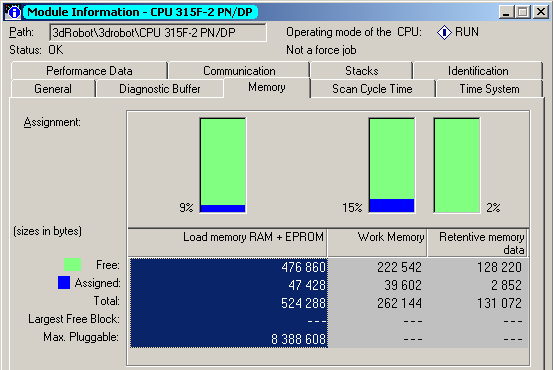
\includegraphics[width=0.6\textwidth]{obrazki/memory.PNG} \caption{Wykorzystanie pamięci sterownika} \label{memory} \end{figure}

\subsection{Specyfikacja zewnętrzna}
Specyfikacja zewnętrzna przedstawiona w dalszej części podrozdziału zawiera opis, jak korzystać z~oprogramowania wgranego do sterownika przez jego autora. Opisane zostało, jak ustawiać odpowiednie zmienne, aby~uzyskać żądany efekt.

Lista zmiennych wejściowych i wyjściowych wymieniana między sterownikiem a modelem została już opisana w~pierwszym rozdziale, w~Tablicach~\ref{in} oraz~\ref{out}. Pozostałe zmienne znajdują się w wewnętrznej pamięci sterownika.

Oprogramowanie może sterować modelem w~sposób automatyczny lub ręczny. Tryb automatyczny w~trybie obsługi magazynu zostanie opisany w podrozdziale 2.1.2. Tryb ręczny może być realizowany przy pomocy zadajnika podpiętego do sterownika lub przy pomocy przycisków umieszczonych na odpowiednim ekranie wizualizacji. W~trybie tym o~pracy robota decydujący jest stan przycisków. Dopuszczalne są wszystkie możliwe ruchy w~przedziale od wyłącznika krańcowego do wartości maksymalnej.

Sterowanie przy pomocy pilota podłączonego do sterownika odbywa się za pomocą 4~przycisków monostabilnych do załączania silników oraz 4~przełączników bistabilnych do wybierania kierunku. Podobne do sterowania pilotem jest sterowanie ręczne z~poziomu wizualizacji, polegające na odpowiednim modyfikowaniu bitów: M11.0~-~M11.7.

W automatycznym trybie pracy kluczową rolę odgrywają 4~zmienne: \emph{LiftEndPos}, \emph{GrabEndPos}, \emph{ArmEndPos} oraz \emph{RotateEndPos} typu INT, które wskazują na pozycje docelowe silników. Są one podawane do bloków FB1 odpowiadających kolejnym silnikom. O tym, czy wybrany silnik może się w~danym momencie poruszać czy nie decydują flagi odpowiednio ustawione przez blok FB9. 

Ważnym elementem jest kolejka obsługiwana w~trybie automatycznym. Indeksy przechowywane są w~przestrzeni od DB6.DBW0 do DB6.DBW202, a~związane z~nimi bezpośrednio zmienne typu bool - w przestrzeni od DB6.DBX202.0 do DB6.DBX216.0. Z kolejką tą związana jest dodatkowo zmienna \emph{CurrentIndex} określająca jej długość.

Kolejną przestrzenią adresową jest blok DB5, który jest reprezentacją w pamięci sterownika modelu magazynu i informacji o nim. Od adresu DB5.DBX0.0 znajduje się 26-elementowa tablica określająca zajętość poszczególnych komórek magazynu. Następnie od adresu DB5.DBW4 dostępna jest dwuwymiarowa tablica 26x3 przechowująca pozycję poszczególnych komórek magazynu. W~przestrzeni zaczynającej się pod adresem DB5.DBB160 znajduje się 26-elementowa tablica zmiennych typu DATE\_AND\_TIME przechowująca datę ostatniego dostępu do komórki. Dodatkowo w przestrzeni tej mamy dostępną pod adresem DB5.DBB368 zmienną przechowującą aktualną datę oraz godzinę w sterowniku, odświeżaną przy każdym przebiegu bloku OB1.

\subsection{Specyfikacja wewnętrzna}
Podrozdział specyfikacja wewnętrzna opisuje sposób rozwiązania przez autora kwestii sterowania modelem przy użyciu dostępnego na~stanowisku sterownika oraz poszczególnych trybów sterowania.
W~tworzeniu oprogramowania zostały wykorzystane następujące języki programowania:
\begin{itemize} 
\item język drabinkowy (Ladder), wykorzystany do stworzenia głównych elementów programu,
\item S7-SCL, który został zastosowany do korzystania z tablic. Niestety do korzystania z nich nie można zastosować języka LAD, ponieważ nie da się w~nim odwoływać do elementów tablicy przez indeksy będące zmiennymi, a~jedynie przez stałe. Po zapoznaniu się z~dokumentacją okazało się, że~taka możliwość istnieje w~języku STL, ale jest to metoda skomplikowana w~implementacji. Właśnie dlatego najlepszym i~najprostszym rozwiązaniem okazuję się S7-SCL, który jest kompilowany do kodu w~języku STL.
\end{itemize} 
Istotne fragmenty programu aplikacyjnego:
\begin{itemize} 
\item blok funkcyjny FB1 - blok sterujący pracą poszczególnych silników,
\item blok funkcyjny FB8 - blok zawierający implementację kolejki FIFO,
\item blok funkcyjny FB9 - blok analizujący stan modelu i ustawiający zmienne zezwalające na ruch silników,
\item blok funkcyjny FB10 - blok przetwarzający zadania z kolejki na odpowiednie dane (operuje na odpowiednich tablicach),
\item blok funkcyjny FB11 - blok zwracający indeks i zmienną bool najbliższego lub najdalszego elementu,
\item blok funkcyjny FB12 - blok zwracający indeks i zmienną bool najmłodszego lub najstarszego elementu.
\end{itemize} 
\indent
\indent Wszystkie wymienione bloki zostaną szczegółowo opisane w kolejnych podrozdziałach.
\vspace*{-9mm}
%dokładniejszy opis poszczególnych bloków w kolejnych podrozdziałach
\subsubsection{Blok FB1}
Najważniejszą częścią oprogramowania jest blok funkcyjny~FB1. Wszystkie zmienne wejściowe oraz wyjściowe dla tego bloku zostały zebrane w Tablicah~\ref{fb1datain}~oraz~\ref{fb1dataout}. Do~działania wykorzystuje~on zestaw danych wewnętrznych. Jako parametry wejściowe bloku, oprócz zmiennych z~modułu~I/O sterownika, podajemy typ aktualnego trybu, maksymalną dopuszczalną wartość wewnętrznego licznika, pozycję docelową w~trybie automatycznym oraz~zmienne \emph{Enable} i \emph{ResetSequence}. Ostatnie dwie zmienne odpowiadają za~to, aby~ruchy w~trybie automatycznym i resetowanie wykonywane były w~odpowiedniej kolejności. Na~wyjściu mamy tylko połączenia dla~zmiennych z~tablicy Symbols oraz~flagę osiągnięcia pozycji docelowej przez dany silnik.

\begin{table}[!htb]
\begin{center}
\begin{tabular}{|c|c|p{8.9cm}|}\hline
Nazwa & Typ & Opis  \\
zmiennej &  zmiennej &   \\\hline
StopSensor & Bool & Sygnał z odpowiedniej krańcówki \\\hline   
EngineCounter & Bool & Sygnał z impulsatora obrotów\\\hline   
CounterMax\_I & Int & Maksymalna wartość licznika typu Int \\\hline   
EndPosition & Int & Pozycja docelowa \\\hline   
Automat & Bool & Tryb automatyczny \\\hline   
ManualWorkDirection & Bool & Start w trybie ręcznym z                                   pilota \\\hline   
ManualWorkStart & Bool & Start w trybie ręcznym z                               wizualizacji \\\hline   
VisualWorkDirection & Bool & Kierunek w trybie ręcznym                                   z pilota \\\hline   
VisualWorkStart & Bool & Kierunek w trybie ręcznym                               z wizualizacji \\\hline   
CounterForState & Counter & Licznik wewnętrzny z aktualną pozycją \\\hline   
Enable & Bool & Sygnał zezwalający na                                                  inkrementację \\\hline   
ResetSequence & Bool & Zmienna pozwalająca na sekwencyjny reset \nobreak{modelu} \\\hline   
VisualPilot & Bool & Zmienna określająca tryb pracy manualnej \break z~pilota~lub wizualizacji \\\hline   
\end{tabular}
\end{center}
\vspace*{-6mm}
  \caption{Zmienne wejściowe do bloku FB1}
	\label{fb1datain}
\end{table}

\begin{table}[!htb]
\begin{center}
\begin{tabular}{|c|c| p{10cm} |}\hline
Nazwa & Typ & Opis  \\
zmiennej &  zmiennej &   \\\hline
EngineOnOff & Bool & Włączenie/wyłączenie                             silnika \\\hline   
EngineDirection & Bool & Kierunek pracy silnika \\\hline   
MinValue & Bool & Sygnał osiągnięcia                           minimum \\\hline   
MaxValue & Bool & Sygnał osiągnięcia                           maksimum \\\hline   
ReachPosition & Bool & Sygnał osiągnięcia                                pozycji docelowej \\\hline   
ResetFinish & Bool & Sygnał zakończenia                                resetu danego silnika \\\hline   
\end{tabular}
\end{center}
\vspace*{-6mm}
  \caption{Zmienne wyjściowe z bloku FB1}
	\label{fb1dataout}
\end{table}

Blok FB1 jest wywoływany w bloku OB1 z~odpowiednimi parametrami, niezależnie dla poszczególnych 4~silników. Przykładowe wywołanie znajduje się na Rysunku~\ref{ob1}. Na rysunku łatwo można zaobserwować, że do bloku podane są wszystkie niezbędne informacje dla danego silnika oraz 2~wspólne dla wszystkich silników sygnały informujące o~aktualnym trybie pracy modelu.
\begin{figure}[!htb] 	\centering 	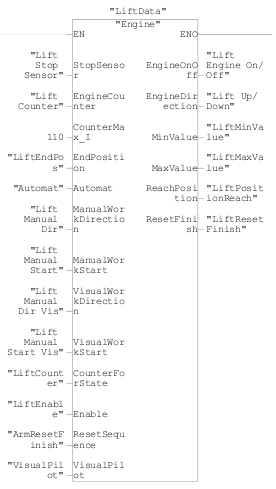
\includegraphics[width=0.58\textwidth]{obrazki/ob1.png} 	\caption{Przykładowe wywołanie FB1 w OB1 dla silnika Lift} \label{ob1} \end{figure} 

Istotnymi fragmentami bloku FB1 są 3~gałęzie programu: licznik wewnętrzny, decyzja o~kierunku oraz decyzja o~załączeniu.
Bardzo istotnym warunkiem wpływającym na pracę silnika jest jego położenie. Jeśli silnik osiąga wartość maksymalną lub minimalną to przerywa swoją pracę. Warunkiem koniecznym do określenia tej pozycji jest wykorzystanie licznika do zliczania impulsów z~modelu i~jego odpowiednia inkrementacja lub dekrementacja. Tak działający licznik przedstawia Rysunek~\ref{licznik}.
\begin{figure}[!htb] 	\centering 	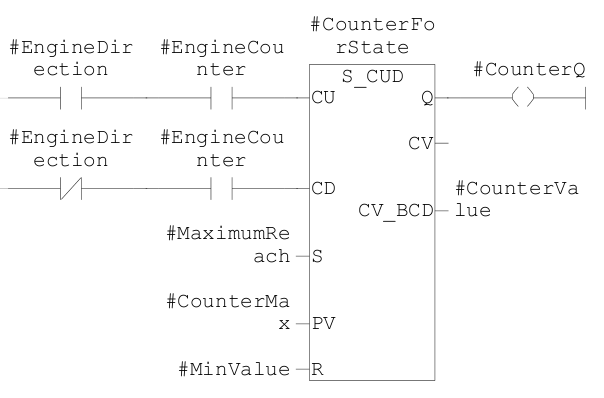
\includegraphics[width=0.5\textwidth]{obrazki/fb1licznik.png} 	\caption{Licznik wewnętrzny dla silnika w bloku FB1} \label{licznik} \end{figure} 

Decyzja dotycząca kierunku jest podejmowana zależnie od trybu pracy, co zaobserwować można na Rysunku~\ref{kierunek}. W~przypadku trybu automatycznego decydująca jest bieżąca pozycja oraz pozycja docelowa. Kierunek jest ustawiany tak, aby załączony silnik zmierzał do~pozycji docelowej. W~przypadku trybów manualnych decydujące są stany przycisków przy sterowaniu z~pilota lub zmienne przy sterowaniu z~wizualizacji. Jeżeli została podjęta decyzja o~załączeniu silnika to stan przycisku (zmiennej) jest wpisywany do zmiennej statycznej \emph{EngineDirectionManual}, która jest następnie zsumowana logicznie ze zmienną \emph{EngineDirectionAuto}, dając w~wyniku decyzję o~kierunku.
\begin{figure}[!htb] 	\centering 	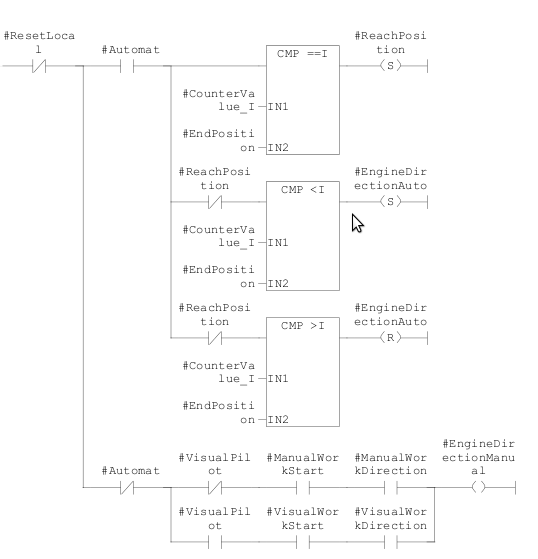
\includegraphics[width=0.66\textwidth]{obrazki/fb1kierunek.png} \caption{Fragment bloku FB1 wybierający kierunek pracy silnika} \label{kierunek} \end{figure} 

Część decydująca o~załączeniu silnika jest bardzo rozbudowana. Jest to przykład załączenia z~podtrzymaniem. Zależnie od trybu pracy sprawdzane są inne warunki. W~przypadku trybu automatycznego ważna jest zmienna \emph{Enable}, która decyduje o~załączeniu wybranego silnika, co pozwala na częściową pracę sekwencyjną. Silnik pracuje w~kierunku krańcówki aż do~jej osiągnięcia, a w~kierunku od krańcówki aż~do osiągnięcia swojego maksimum, chyba że~wcześniej zostanie osiągnięta pozycja docelowa. W~ręcznych trybach pracy głównym warunkiem decydującym o~załączeniu zależnie od kierunku są wartość maksymalna licznika lub krańcówka. Wspólnym dla obu trybów warunkiem pozwalającym zatrzymać pracę silnika jest ustawienie zmiennej \emph{EmergencyStop} na wartość \emph{true}. Tą rozbudowaną i skomplikowaną gałąź prezentuje Rysunek~\ref{onoff}.
\begin{figure}[!htb] 	\centering 	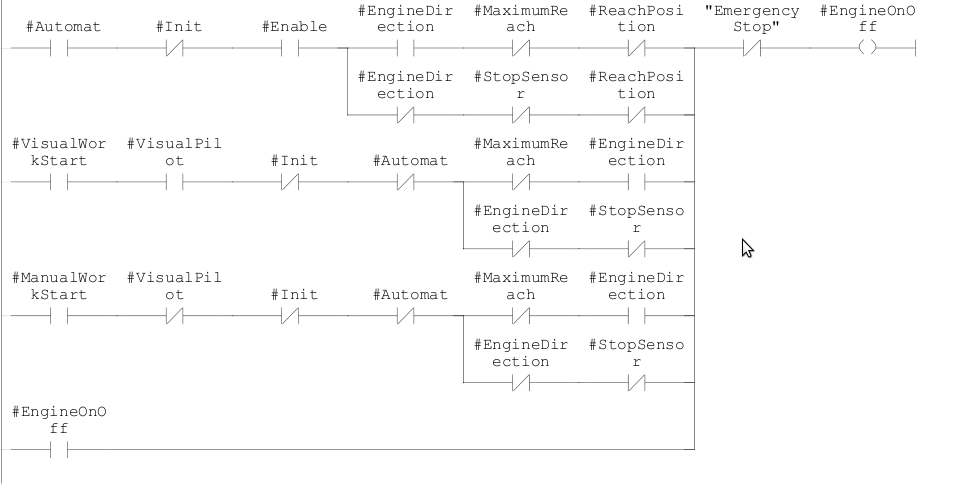
\includegraphics[width=0.95\textwidth]{obrazki/fb1wlwyl.png} 	\caption{Fragment bloku FB1 decydujący o załączeniu silnika} \label{onoff} \end{figure} 

\subsubsection{Blok FB8}
W trybie automatycznym podczas obsługi magazynu praca odbywa się na zasadzie zadań do wykonania. Na zadanie takie składa się indeks komórki w magazynie oraz zmienna typu bool, która decyduje o ruchu chwytaka (zaciskanie lub zwalnianie). Indeks jest następnie przetwarzany w odpowiednim bloku na położenie komórki w modelu magazynu. 

Bardzo ważnym blokiem funkcyjnym jest blok zarządzający kolejką zadań do wykonania w trybie automatycznym. Na wejściu znajdują się: dodawany do kolejki indeks oraz zmienna decydująca o zamknięciu lub otwarciu chwytaka. Na wyjściu mamy zmienne takie same jak na wejściu, ale przepuszczone już przez kolejkę. Zmienne wejściowo-wyjściowe to 2~flagi żądania, odpowiednio: dodania do kolejki lub pobrania z niej elementu oraz 2~flagi potwierdzające wykonanie żądania. Dodatkowo w~bloku tym występuje zmienna wewnętrzna stanowiąca indeks w~tablicy. 
\newpage
\begin{lstlisting}[caption={FB8 - Zarządzanie kolejką}]
FUNCTION_BLOCK FB8

VAR_INPUT
    AddedBool: BOOL;
    AddedIndex: INT;
END_VAR     

VAR_OUTPUT 
    WarehouseBool: BOOL;
    WarehouseIndex: INT;
END_VAR  

VAR_IN_OUT
    Request: BOOL;
    Add: BOOL;
    RequestAck: BOOL;
    AddAck: BOOL;
END_VAR  

VAR
    Index: INT ;
END_VAR

BEGIN
IF Add = true & Queue.CurentIndex <= 100 THEN
    IF AddedIndex >= 0 AND AddedIndex < 26 THEN
        Queue.QueueIndex[Queue.CurentIndex] := AddedIndex;
        Queue.QueueBool[Queue.CurentIndex] := AddedBool;
        Queue.CurentIndex := Queue.CurentIndex + 1;
        Add := false;
        AddAck := true;
    ELSE
        Error.IndexError := 'Indeks spoza zakresu';    
        Error.IndexErrorPres := true;
    END_IF;
ELSIF Queue.CurentIndex >= 100 THEN   
    Error.QueueError := 'Przepelniona Kolejka';
    Error.QueueErrorPres := true;    
END_IF;

IF Request = true & Queue.CurentIndex > 0 THEN
    IF Queue.QueueIndex[0] <> -1 THEN        
        WarehouseIndex := Queue.QueueIndex[0];
        WarehouseBool := Queue.QueueBool[0];
            FOR Index := 0 TO Queue.CurentIndex DO
                Queue.QueueIndex[Index] := Queue.QueueIndex[Index+1];
                Queue.QueueBool[Index] := Queue.QueueBool[Index+1]; 
            END_FOR;        
        Queue.QueueIndex[Queue.CurentIndex] := 0;
        Queue.QueueBool[Queue.CurentIndex] := false;
        Queue.CurentIndex := Queue.CurentIndex - 1;
        Request := false;
        RequestAck := true;
    ELSE
        Error.IndexError := 'Bledny indeks';    
        Error.IndexErrorPres := true;            
    END_IF;    
ELSIF Queue.CurentIndex = 0 THEN
    Request := false;   
    RequestAck := false;     
    Error.QueueError := 'Kolejka jest pusta';    
    Error.QueueErrorPres := true;
END_IF;
END_FUNCTION_BLOCK
\end{lstlisting}
\subsubsection{Blok FB9}
Kolejnym istotnym blokiem jest blok decydujący o~zezwoleniu na pracę poszczególnych silników, pozwalając przez to wykonywać ruchy ramienia w~odpowiedniej kolejności. Blok na wyjściu posiada 4~zmienne stanowiące właściwe zezwolenie na ruch. Decyzja jest podejmowana na podstawie położenia silnika Arm oraz osiągnięcia przez poszczególne silniki swoich pozycji docelowych.
\begin{lstlisting}[caption={FB9 - Zezwolenie na ruch}]
FUNCTION_BLOCK FB9

VAR_INPUT
    ArmCounterl: COUNTER;
END_VAR     

VAR_OUTPUT
    ArmEn: BOOL;
    LiftEn: BOOL;
    RotateEn: BOOL;
    GrabEn: BOOL;            
END_VAR     

BEGIN
    IF AutoTest THEN
        ArmEn := true;
        LiftEn := true;
        RotateEn := true;
        GrabEn := true;
    ELSE     
        IF ArmData.CounterValue_I <= 25 THEN
            ArmEn := true;
            LiftEn := true;
            RotateEn := true;
            GrabEn := false;
        ELSE
            IF LiftPositionReach  AND RotatePositionReach THEN        
                ArmEn := true;   
                LiftEn := false;
                RotateEn := false;
                GrabEn := false;  
            ELSE
                IF ArmData.CounterValue_I > 25 THEN
                    ArmEn := true;
                    LiftEn := false;
                    RotateEn := false;
                    GrabEn := false;
                else
                    ArmEn := false;   
                    LiftEn := true;
                    RotateEn := true;
                    GrabEn := false;              
                END_IF;
            END_IF;    
        END_IF;        
        IF LiftPositionReach & RotatePositionReach & ArmPositionReach THEN
            ArmEn := false;   
            LiftEn := false;
            RotateEn := false;
            GrabEn := true;    
        END_IF;    
    END_IF;           
END_FUNCTION_BLOCK
\end{lstlisting}

\subsubsection{Blok FB10}
Blok funkcyjny FB10 zarządza operacjami wykonywanymi na tablicach związanych z~obsługiwanym magazynem. Na~wejściu mamy zmienne stanowiące wyjście z~kolejki oraz zmienną określającą, że~wykonane zostało ostatnie podzadanie uruchomione przez ten blok. Na~wyjściu mamy zmienne określające, do jakich pozycji mają dojechać silniki. 

Zmienne wejściowo-wyjściowe to żądanie następnego zadania z~kolejki oraz potwierdzenie obsłużenia żądania przez kolejkę. Zmienna tymczasowa jest to wartość zwrócona przez funkcję systemową odczytu bieżącej daty oraz godziny. Zmienna wewnętrzna \emph{DoneCount} przechowuje informację o tym, ile podzadań zostało wykonanych. 
\begin{lstlisting}[caption={FB10 - Operacje na tablicah}]
FUNCTION_BLOCK FB10

VAR_INPUT
    Done: BOOL;
    WarehouseIndex: INT;
    WarehouseBool: BOOL;
END_VAR 

VAR_OUTPUT
    ArmTo: INT;
    LiftTo: INT;
    RotateTo: INT;
    GrabTo: INT;            
END_VAR

VAR_IN_OUT
    NextRequest: BOOL;
    NextRequestACK: BOOL;
END_VAR  
 
VAR_TEMP
    SFC1_Ret_val: INT;    
END_VAR

VAR
    DoneCount: INT;
    LoadNext: BOOL;
END_VAR
    
BEGIN

IF NextRequestACK = true THEN
    NextRequest := false;
    NextRequestACK := false;
    DoneCount := 0;    
    ArmTo := 22;
    IF WarehouseBool THEN
        LiftTo := Warehouse.WarehousePosition[WarehouseIndex, 2];    
    ELSE 
        LiftTo := Warehouse.WarehousePosition[WarehouseIndex, 2]-3;
    END_IF;  
    RotateTo := Warehouse.WarehousePosition[WarehouseIndex, 3];
    LoadNext := true;
END_IF;

IF DoneCount = 1 THEN
    ArmTo := Warehouse.WarehousePosition[WarehouseIndex, 1];
    IF WarehouseBool THEN
        LiftTo := Warehouse.WarehousePosition[WarehouseIndex, 2];    
    ELSE 
        LiftTo := Warehouse.WarehousePosition[WarehouseIndex, 2]-3;
    END_IF;        
    RotateTo := Warehouse.WarehousePosition[WarehouseIndex, 3];
    GrabTo := BOOL_TO_INT(WarehouseBool) * 19;
END_IF;
    
IF DoneCount = 2 THEN
    Warehouse.WarehouseBool[WarehouseIndex] := NOT WarehouseBool;
    SFC1_Ret_val := SFC1(CDT := Warehouse.WarehouseDateTime[WarehouseIndex]);
    DoneCount := 0;
    IF Queue.CurentIndex > 0 THEN
        NextRequest := true;
        LoadNext := false;
    ELSE
        Error.QueueError := 'Kolejka jest pusta';  
    END_IF;
END_IF;

IF Done = true & LoadNext THEN
    DoneCount := DoneCount + 1;    
END_IF;       
END_FUNCTION_BLOCK
\end{lstlisting}
\subsubsection{Blok FB11}
Blok FB11 w wyniku działania zwraca indeks komórki w magazynie oraz powiązaną z~nim zmienną typu bool, które pozwalają wybrać najdalej lub najbliżej położony element. Wskazuje on pustą lub zajętą komórkę magazynu, zależnie od zmiennych wejściowych. Zależnie od wartości zmiennej \emph{FarNear} wybierana jest najdalej lub najbliżej położona komórka, natomiast zmienna \emph{BoolGrab} decyduje o~tym, czy szukamy wolnej czy zajętej komórki magazynu. 

W wyniku działania blok ustawia na wyjściu zmienne związane z~wybraną komórką magazynu oraz flagę żądania dodania uzyskanego wyniku do kolejki zadań. Zmienna \emph{MyEn} decyduje o tym, czy ten blok zostaje aktywowany czy nie. Zmienna index jest zmienną wewnętrzną wykorzystywaną w~pętlach FOR.
\begin{lstlisting}[caption={FB11 - Funkcja wybiera najdalszą lub najbliższą komórkę}]
FUNCTION_BLOCK FB11

VAR_INPUT
    FarNear: BOOL;
END_VAR 

VAR_OUTPUT
    IndexSel: INT;
    AddQueue: BOOL;
END_VAR
 
VAR_IN_OUT
    MyEn: BOOL;
    BoolGrab: BOOL;
END_VAR  

VAR
    Index: INT;
END_VAR    
    
BEGIN
IF MyEn = true THEN    
    IF FarNear = true & BoolGrab = true THEN    
        FOR Index := 1 TO 24 DO
            IF Warehouse.WarehouseBool[Index] = true THEN
                IndexSel := Index;
                EXIT;
            ELSE
                IndexSel := -1;                
            END_IF;
        END_FOR;        
    END_IF;
    
    IF FarNear = false & BoolGrab = true THEN
        FOR Index := 24 TO 1 BY -1 DO
            IF Warehouse.WarehouseBool[Index] = true THEN
                IndexSel := Index;
                EXIT;
            ELSE
                IndexSel := -1;                                
            END_IF;            
        END_FOR;
    END_IF;
    
    IF FarNear = true & BoolGrab = false THEN
        FOR Index := 1 TO 24 DO
            IF Warehouse.WarehouseBool[Index] = false THEN
                IndexSel := Index;
                EXIT;
            ELSE
                IndexSel := -1;                                                
            END_IF;            
        END_FOR;
    END_IF;
    
    IF FarNear = false & BoolGrab = false THEN
        FOR Index := 24 TO 1  BY -1 DO
            IF Warehouse.WarehouseBool[Index] = false THEN
                IndexSel := Index;
                EXIT;
            ELSE
                IndexSel := -1;                                                
            END_IF;            
        END_FOR;
    END_IF;   
    MyEn := false;
    AddQueue := true;
END_IF;       
END_FUNCTION_BLOCK
\end{lstlisting}
\subsubsection{Blok FB12}
Blok FB12 w wyniku działania zwraca indeks komórki w magazynie oraz powiązaną z~nim zmienną typu bool, które pozwalają wybrać najstarszy lub najmłodszy element tablicy. Wskazuje on zajętą komórkę magazynu. Zależnie od wartości zmiennej \emph{SmallestGreatest} wybierana jest najmłodsza lub najstarsza zajęta komórka. 

W wyniku działania blok ustawia na wyjściu zmienne związane z~wybraną komórką magazynu oraz flagę żądania dodania uzyskanego wyniku do kolejki zadań. Zmienna \emph{MyEn} decyduje o~tym, czy ten blok zostaje aktywowany czy nie. Zmienna index jest zmienną wewnętrzną wykorzystywaną w~pętlach FOR. \emph{IndexTemp} jest zmienną pomocniczą stanowiącą tymczasowy indeks przy wybieraniu elementu końcowego.
\begin{lstlisting}[caption={FB12 - Funkcja wybiera najmłodszą lub najstarszą zajętą komórkę}]
FUNCTION_BLOCK FB12

VAR_INPUT
    SmallestGreatest: BOOL;
END_VAR 

VAR_OUTPUT
    IndexSelected: INT;
    BoolSelected: BOOL;
    AddQueue: BOOL;    
END_VAR
 
VAR_IN_OUT
    MyEn: BOOL;
END_VAR  
 
VAR
    Index: INT;
END_VAR
    
VAR_TEMP
    IndexTemp: INT;
END_VAR 
       
BEGIN
IF MyEn = true THEN    
    
    IF SmallestGreatest = false THEN    
        FOR Index := 1 TO 24 DO        
            IF Warehouse.WarehouseBool[Index] = true AND FC28(DT1 := Warehouse.WarehouseDateTime[Index], DT2 := DT#1990-01-01-12:00:00.00) THEN
                IndexTemp := Index;
                EXIT;
            ELSE
                IndexTemp := -1;
            END_IF;
        END_FOR;  
        IF IndexTemp <> -1 THEN                   
            FOR Index := 1 TO 24 DO        
                IF Warehouse.WarehouseBool[Index] = true then
                    IF FC14(DT1 := Warehouse.WarehouseDateTime[Index], DT2 := Warehouse.WarehouseDateTime[IndexTemp]) THEN
                        IndexTemp := Index;            
                    END_IF;
                END_IF;
            END_FOR;        
        END_IF;           
    END_IF;
    
    IF SmallestGreatest = true THEN
        FOR Index := 1 TO 24 DO        
            IF Warehouse.WarehouseBool[Index] = true AND FC28(DT1 := Warehouse.WarehouseDateTime[Index], DT2 := DT#1990-01-01-12:00:00.00) THEN
                IndexTemp := Index;
                EXIT;
            ELSE
                IndexTemp := -1;
            END_IF;
        END_FOR;      
        IF IndexTemp <> -1 THEN                   
            FOR Index := 1 TO 24 DO
                IF Warehouse.WarehouseBool[index] = true then        
                    IF FC23(DT1 := Warehouse.WarehouseDateTime[Index], DT2 := Warehouse.WarehouseDateTime[IndexTemp]) THEN
                        IndexTemp := Index;
                    END_IF;            
                END_IF;            
            END_FOR;
        END_IF;            
    END_IF;
    MyEn := false;
    IndexSelected := IndexTemp;
    BoolSelected := true;
    AddQueue := true;
END_IF;    
END_FUNCTION_BLOCK
\end{lstlisting}
 %
\lstset{language=VBScript,
        basicstyle=\footnotesize\ttfamily,
        breaklines=true,
        tabsize=2,
        numbers=left,
        numberstyle=\tiny,
        numbersep=7pt,
        showspaces=false,
        keywordstyle=\color{Blue}\textbf,
        commentstyle=\color{Red}\emph,
        showstringspaces=false,
        stringstyle=\color{BurntOrange}
        }
\section{Wizualizacja HMI}
Zaimplementowana przez autora wizualizacja ma na~celu zobrazowanie działania modelu oraz umożliwienie operatorowi wpływania na~jego działanie. Kolejne podrozdziały zawierają opis specyfikacji zewnętrznej oraz wewnętrznej. Część odnosząca się do specyfikacji zewnętrznej jest skróconą instrukcją obsługi użytkownika. Specyfikacja wewnętrzna jest opisem, jak zostały zrealizowane poszczególne elementy~i~w jaki sposób wizualizacja współpracuje ze~sterownikiem.

\subsection{Specyfikacja zewnętrzna}
Specyfikacja zewnętrzna przedstawiona w dalszej części podrozdziału stanowi skróconą instrukcję obsługi wizualizacji oraz opis możliwości oferowanych przez poszczególne ekrany.

Autor projektu wykorzystał w~swojej pracy szereg elementów dostępnych standardowo w~środowisku Simatic WinCC flexible. Podstawowymi elementami sterującymi są przyciski w~trybie tekstowym oraz przeźroczystym. Głównymi obiektami służącymi do prezentacji informacji są: pola tekstowe, pola wejściowo-wyjściowe oraz pola daty i~godziny. Dodatkowo celem uatrakcyjnienia wizualizacji wykorzystane zostały suwaki (ang. \emph{slider}), obrazki oraz zegarek. 

Obsługa tej części projektu jest realizowana za pomocą myszy i~klawiatury podłączonych do~komputera. Za~pomocą klawiatury wybieramy interesujący nas ekran lub wprowadzamy żądaną wartość pozycji docelowej na~ekranie testowania trybu automatycznego.

\subsection{Specyfikacja wewnętrzna}
Wizualizacja komunikuje się z~komputera klasy~PC ze~sterownikiem za~pośrednictwem protokołu Ethernet w~sieci lokalnej.
Odniesienia do~odpowiednich adresów w~pamięci sterownika dokonywane są za~pomocą nazw symbolicznych zdefiniowanych w~tablicy Tags. Do działania wizualizacja używa tylko jednej zmiennej wewnętrznej i~jest~to zmienna tablicowa \emph{MagazynDTEnable} z elementami typu bool. Elementy te odpowiadają za~wyświetlanie dat oraz godzin na~ekranie ze~stanem magazynu po~kliknięciu na~wybraną komórkę. Obsługa wyświetlania dat polega na tym, że po kliknięciu w wybrane pole ustawiana jest odpowiednia zmienna w~tej tablicy na~wartośc \emph{true}, a~po zwolnieniu klawisza myszki na wartość \emph{false}. Za zmiany te odpowiadają niewidzialne przyciski umieszczone na~tych polach.

Wizualizacja wpływa na pracę sterownika poprzez zmianę pojedynczych bitów za~pomocą umieszczonych na~ekranie przycisków. Wpływa ona również poprzez modyfikowanie wybranych zmiennych odpowiadających pozycjom docelowym lub poprzez dodawanie odpowiednich zadań do~kolejki. Bardziej zaawansowane operacje zostały zrealizowane za~pomocą skryptów napisanych w~języku VBScript, które są bardzo prostą i~szybką opcją wykonywania bardziej zaawansowanych czynności.  %
\section{Uruchamianie i testowanie}
Rozdział ten zawiera podsumowanie przebiegu prac nad projektem. Opisane zostaną tu~wszelkie poważne problemy, które wystąpiły w~czasie realizacji projektu. Ponadto zawarto~tu opis przebiegu procesu testowania.

%\subsection{Przebieg testowania}
%W procesie weryfikacji poprawności działania projektu zastosowano testowanie wstępujące. 
%
%Głównym testerem był autor projektu więc większość testów przebiegała na zasadzie białej skrzynki (ang. \emph{white box}), bardzo często z~użyciem podglądu stanu w środowisku TwinCAT System Manager. Takie testowanie pozwala stosunkowo łatwo wyszukać źródło błędu i~je wyeliminować.
%
%Autor kilka razy przeprowadzał testy stosując metodę czarnej skrzynki (ang. \emph{black box}), nie~biorąc pod uwagę zależności wykonywanych czynności, od~realizowanego przez sterownik kodu. Kilkukrotnie w czasie realizacji projektu do testów zgłaszały się osoby trzecie, które były nim zaciekawione. Testy wykonane przez takie osoby są niezwykle cenne ze względu na dużą nieprzewidywalność oraz całkowitą niezależność działań od rozwiązań ze~względu na~brak ich znajomości.
%
%W~czasie realizacji autor stosował testowanie oparte na dwóch metodach analizy. Testowanie oprogramowania można wykonywać pod kątem analizy statycznej i~dynamicznej. Analiza statyczna polega na~sprawdzaniu kodu źródłowego i~znajdowaniu w~nim błędów bez uruchamiania sprawdzanego kodu. Ta~metoda była stosowana poza laboratorium, gdzie brak był dostępu do sterownika i~modelu. Podczas analizy dynamicznej oprogramowanie jest uruchamiane i~badane pod kątem ścieżki przebiegu i~czasu wykonywania. Ta metoda z~kolei była najważniejsza i~często wyniki tych testów były zaskakujące w~stosunku do~przeprowadzonych wcześniej z~zastosowaniem analizy statycznej.
%
%Ostatnim etapem testów były~te przeprowadzone w~obecności promotora oraz te wykonane przez niego. Ostatecznie oprogramowanie zostało zatwierdzone i~uznane za spełniające wszystkie wstępne założenia przedstawione w~podrozdziale 1.2.
%\newpage
\subsection{Napotkane problemy}
Podczas tworzenia projektu napotkane i~przeanalizowane zostały następujące problemy:
\begin{itemize}
\item Problem z automatycznym uruchamianiem stworzonego projektu PLC:\\[1mm]
Po utworzeniu oprogramowania sterownika~PLC~oraz po odpowiednim skonfigurowaniu go w oprogramowaniu TwinCAT System Manager tj. linkowaniu zmiennych programu do~odpowiednich fizycznych wejść oraz wyjść modelu oraz aktywowaniu tak przygotowanej konfiguracji, które z~kolei wymusza zresetowanie systemu nie~następuje uruchomienie projektu sterownika PLC. W początkowej fazie autor przełączał się na oprogramowanie TwinCAT PLC Control gdzie logował się do~sterownika i~ręcznie uruchamiał stworzony przez siebie kod. Niestety to~rozwiązanie na~dłuższą metę okazało~się męczące i~czasochłonne. Okazało się, że~w~sterownikach firmy Beckhoff trzeba w~specjalny sposób przygotować oprogramowanie, które ma~być uruchamiane w~sposób automatyczny, tzn. trzeba utworzyć projekt, który jest bootowalny. Początkowo takie podejście wydało się autorowi bardzo dziwne, ale po~dłuższym zastanowieniu oraz kilku rozmowach z~bardziej doświadczonymi w~branży osobami okazało się, że~ma~ono swoje plusy. Przykładowo w~przypadku tworzenia oprogramowania w~fazie rozwojowej reset urządzenia pozwala przerwać całkowicie wykonywanie oprogramowania zawierającego błędy mające destrukcyjny wpływ na~model lub w~praktyce na~obiekt przemysłowy. Po~zastosowaniu nowej metody uruchamianie~i testowanie tworzonego oprogramowania stało~się zdecydowanie prostsze.

\item Problem z~wykryciem jednego z~silników:\\[1mm]
aa

\item Utrata komunikacji z~jednym ze sterowników:\\[1mm]
Przy pewnej modyfikacji konfiguracji stanowiska typu~CX związanej z~próbą uruchomienia silników została utracona komunikacja z urządzeniem. Dokładnie przestało ono odpowiadać na~poprzednim adresie. Sytuacja była o~tyle dziwna, że system na urządzeniu działał całkowicie normalnie. Po~podpięciu zewnętrznego monitora okazało się, że w systemie operacyjnym karty sieciowe są skonfigurowane prawidłowo oraz udaje się nawiązać połączenie i~uzyskać żądany adres (konfiguracja adresów jest statyczna). Próby wykorzystania programu ping nie~dały początkowo żadnego efektu, ponieważ urządzenie nie odpowiadało. W licznych próbach i~pomysłach udało się ustalić, że urządzenie podczas uruchamiania (dokładnie podczas uruchamiania systemu operacyjnego) odpowiada na kilka zapytań (od 4 do 6 w kilku próbach), podobnie w momencie zamykania systemu. To~odkrycie zasugerowała autorowi, że~coś blokuje, przekonfigurowywuje lub wywłaszcza urządzenia. Pierwszy został przeanalizowany autostart systemu Windows lecz okazał się on pusty. Pojawił się pomysł przywrócenia urządzenia do ustawień fabrycznych lecz nie~udało się odnaleźć takiej możliwości. Problem udało się rozwiązać uruchamiając w~systemie operacyjnym standardowy menadżer plików (w~tym przypadku explorer), odnajdując stworzone pliki konfiguracji TwinCAT i~usuwając~je. ($\backslash Hard Disk\backslash TwinCAT\backslash Boot\backslash$)

\end{itemize}
\indent
\indent Wszystkie problemy zostały rozwiązane i~w~ostatecznej wersji oprogramowania nie wpływają one w~negatywny sposób na~pracę modelu.
 %
\section{Wnioski}
Protokół EtherCAT jest rozwiązaniem zdecydowanie bardzo nowoczesnym, zaawansowanym oraz pomysłowym. Pozwala bardzo dobrze wykorzystać wzrastające moce obliczeniowe sterowników~PLC, przy zachowaniu wszelkich rygorów czasowych.
Zdecydowanie ogromny wpływ na~tak szybki rozwój ma~fakt, że~technologia jest bardzo otwarta i~postawiona na~współpracę wszystkich zainteresowanych rozwojem stron. Olbrzymim plusem jest fakt wykorzystania standardowej struktury Ethernetu co upraszcza proces integracji w obrębie jednego systemu obu standardów.

Temat zdecydowanie nadaje~się do~pogłębiania i~dalszych badań. Autor dopuszcza taką możliwość w~ramach prac badawczych w~toku swoich studiów doktoranckich. Zarówno same sterowniki firmy Beckhoff oparte o koncepcję ,,soft PLC'' jak i sam badany protokół EtherCAT są na~tyle rozbudowane i rozwojowe, że zawsze znajdzie się jakiś aspekt do~przeanalizowania od strony teoretycznej i~eksperymentalnej. W momencie powstawania niniejszej pracy dwa bardzo interesujące kwestie wydają się autorowi ciekawą postawą do przeprowadzenia badań.

Po pierwsze przetestowanie elementów sieci EtherCAT pochodzących od innych producentów. 
Jak już zostało to opisane w rozdziale zawierającym analizę tematu węzły EtherCAT mogą być realizowane na wiele sposobów zależnie od wymagań funkcjonalnych. Autor bardzo chętnie podjąłby badania mające na celu zaprojektowanie własnego układu cyfrowych wejść/wyjść i porównanie takiego rozwiązania z dostępnymi na rynku, aby wyznaczyć stosunek jakości do kosztów. W dalszym etapie zdecydowanie warto~by przyjrzeć się bardziej elastycznym i rozbudowanym rozwiązaniom pozwalającym na realizację bardziej zaawansowanych węzłów.
Interesująca wydaje się możliwość konstruowania zupełnie od podstaw węzłów o dowolnej funkcjonalności. Dzięki temu można by spróbować zbudować węzeł eksperymentalny mający za zadanie tylko monitorowanie przepływających przez niego ramek i~ich ewentualne gromadzenie. Być może taka analiza krążących w sieci ramek pozwoliłaby wykryć jakieś interesujące właściwości lub zachowania charakterystyczne dla omawianego protokołu.

Zdaniem autora najbardziej interesujące pod względem badawczym są właśnie jednostki wyposażone w~procesor dedykowany do~realizacji bardziej złożonych zadań niezależnie od działania protokołu. Ciekawym rozwiązaniem jest oferowany przez firmę Texas Instruments mikrokontroler z rdzeniem ARM Cortex-A8 z rodziny Sitara AM335x. Być może rozwiązania firm wchodzących w~skład ETG okażą się lepsze lub gorsze pod względem szybkości w porównaniu do pierwszych twórców protokołu.

Drugim ciekawym rozwiązaniem i pomysłem na~które autor natrafił w~sieci w~czasie analizy tematu, rozwiązywania problemów oraz pisania niniejszej pracy jest EtherLab. Jest to technologia łącząca sprzęt i oprogramowanie w celach testowych oraz do~sterowania procesów przemysłowych. Jest~to niejako technika zbudowana z~dobrze znanych i~niezawodnych elementów.
EtherLab pracuje jako działający w czasie rzeczywistym moduł jądra otwartego systemu Linux, który komunikuje się z urządzeniami peryferyjnymi poprzez protokół EtherCAT. Rozwiązanie jest całkowicie darmowe i otwarte co na~pewno jest jego olbrzymią zaletą. Można zdecydować się na pobranie sobie wszystkich komponentów i~ich samodzielne uruchomienie lub zakup gotowego preinstalowanego zestawu startowego bezpośrednio od twórców. 
Oprogramowanie całego zestawu może zostać wygenerowane przy użyciu Simulinka/RTW lub napisane ręcznie w C. Następnie tak przygotowane jest uruchamiane w środowisku kontrolującym proces (jądro Linuksa oraz moduł czasu rzeczywistego) komunikującym się z ,,obiektem przemysłowym'' poprzez EtherCAT. Dodatkowo można rozszerzyć możliwości całego zestawu poprzez Ethernet TCP/IP dołączając interfejs użytkownika (ang. Frontend) w wersji dla Linuksa lub Windowsa albo jeden z innych dodatkowych serwisów. Przykładowe serwisy to:
\begin{itemize}
\item Raportowanie poprzez SMS,
\item Zdalne usługi: Internet, ISDN, DSL,
\item Usługi sieciowe: Web, DHCP, Drukowanie,
\item Logowanie danych (ang. data logging).
\end{itemize}
Jeżeli autor będzie miał taką możliwość to~na~pewno chętnie przyjrzy się tej koncepcji ze~względu na swoją sympatię do~systemu Linux oraz wszystkich rozwiązań go wykorzystujących. Ciekawe wydają~się badania wydajności takiego rozwiązania oraz porównanie ich z drogimi rozwiązaniami komercyjnymi.
 %
\section{Bibliografia}
Literatura, która została wykorzystana przez autora w czasie powstawania projektu, którą opisuje niniejsza dokumentacja.

\begin{thebibliography}{99}
\bibitem{plc1} 
Jerzy Kasprzyk: 
\emph{"Programowanie sterowników przemysłowych"},
Wydawnictwa Naukowo-Techniczne WNT, 
Warszawa, 
2007.      

\bibitem{plc2} 
\emph{"Programowalne sterowniki PLC w systemach sterowania przemysłowego"}, 
Politechnika Radomska, 
Radom,
2001.

\bibitem{plc4} 
Andrzej Maczyński:
\emph{„Sterowniki programowalne PLC. Budowa systemu i podstawy programowania”},
Astor, 
Kraków,
2001. 

\bibitem{plc5} 
Zbigniew Seta: 
\emph{„Wprowadzenie do zagadnień sterowania. Wykorzystanie programowalnych sterowników logicznych PLC.”},
MIKOM Wydawnictwo, 
Warszawa,
2002. 

\bibitem{plc6} 
Janusz Kwaśniewski: 
\emph{„Programowalne sterowniki przemysłowe w systemach sterowania”}, 
Wyd. AGH, 
Kraków,
1999.

%\bibitem{beck1} 
%Dokumentacja producenta: 
%\emph{„Servo Drive AX5000”}, 
%28 wrzesień 2012.
%
%\bibitem{kurs1} 
%Materiały szkoleniowe: Rudolf W. Meier:
%\emph{„AX5000 – Motion control for high dynamic positioning”},
%luty 2007.
%
%\bibitem{kurs2} 
%Materiały szkoleniowe:
%\emph{„Pierwsze kroki w TwinCAT System Manager i TwinCAT PLC Control”},
%29 październik 2007.
%
%\bibitem{kurs3} 
%Materiały szkoleniowe:
%\emph{„Podstawy obsługi programów: TwinCAT System Manager i TwinCAT PLC Control”},
%15 grudzień 2006.

\bibitem{art1_etherCAT} 
Andrzej Gawryluk:
\emph{„EtherCAT – to nie takie trudne. Ethernet jako sieć real-time”},
Elektronika Praktyczna, 2/2010.

\bibitem{art2_etherCAT} 
Michał Gosk:
\emph{„Szybkość, niezawodność, doskonała synchronizacja. EtherCAT - system przyszłości.”},
Magazyn Sensor, 1/2013, kwiecień.

\bibitem{art_softPLC}
Krzysztof Oprzędkiewicz:
\emph{,,Realizacja predyktora Smitha na platformie sprzętowo-programowej ,,soft PLC'' bazującej na komputerze klasy PC''},
Automatyka~/~Akademia Górniczo-Hutnicza im. Stanisława Staszica w Krakowie,
2006,
t. 10, z. 2, s. 177--186,
ISSN 1429-3447.

\bibitem{projekt_FPGA}
Rafał Cupek, Piotr Piękoś, Marcin Poczobut, Adam Ziebinski:
\emph{,,FPGA based ,,Intelligent Tap'' device for real-time Ethernet network monitoring''},
Computer Networks, Communications in Computer and Information Science, Springer-Verlag Berlin Heidelberg,
2010,
t. 79, s. 58-66,
ISBN 978-3-642-13860-7.

\bibitem{FPGA_Xilinx}
Dokumentacja producenta: 
\emph{,,ET1815 / ET1817 EtherCAT Slave Controller IP Core for Xilinx FPGAs IP Core Release 2.02a”}, 
Wersja 2.2.1,
1 wrzesień 2008.

\bibitem{FPGA_Altera}
Dokumentacja producenta: 
\emph{„ET1810 / ET1812 EtherCAT Slave Controller IP Core for Altera FPGAs IP Core Release 2.4.0”}, 
Wersja 1.0
15 marca 2011.

\end{thebibliography} %
\section{Spis rysunków, tablic i kodów źródłowych}
\subsection{Spis rysunków}
%\listoffigures
\renewcommand*\numberline[1]{Rysunek\,#1:\indent}
\listoffigures
\subsection{Spis tablic}
\renewcommand*\numberline[1]{Tablica\,#1:\indent}
\listoftables
\subsection{Spis kodów źródłowych}
\renewcommand*\numberline[1]{Kod źródłowy\,#1:\indent}
\lstlistoflistings
\section{Załączniki}
\begin{itemize}
\item Oświadczenie o autorstwie,
\item Płyta CD, na której znajdują się:
\begin{itemize}
\item Kod oprogramowania wewnętrznego TwinCAT PLC Control,
\item Pliki projektu TwinCAT System Manager,
\item Kod wizualizacji oraz pliki projektu !?,
\item Plik wykonywalny wizualizacji !?
\item \LaTeX-owe, TikZ-owe oraz PGF-owe  pliki źródłowe pracy magisterskiej.
\end{itemize}
\end{itemize}
 %
\end{document}
